% A (little more than a) minimal working example
\documentclass[12pt, a4paper]{article}

% Increase tex widht and heigh by 4cm
\addtolength{\textwidth}{4cm}
\addtolength{\oddsidemargin}{-2cm}
\addtolength{\textheight}{4cm}
\addtolength{\topmargin}{-2cm}

% To start out let's include the following packages
\usepackage[utf8]{inputenc} % encoding
\usepackage{hyperref} % for clickable references
\usepackage{xcolor} % custom colors
\usepackage{graphicx} % for including graphics
\usepackage{pgfplots} % for plots and more
\usepackage{tikz} % for drawing and more
\usepackage{booktabs} % for nice tables
\usepackage{amsmath} % math stuff
\usepackage{amsfonts}
\usepackage{amssymb}

\begin{document}
	
	\title{%
		{\bfseries Better Than Worst-Case Computing }\\[1ex] % your title goes here
		{\large\bfseries Why not to miss the typical case} % if you want to use a subtitle...
	}
	\author{Oliver Klöckner} % your name
	
	\date{\vspace{-5ex}} % dirty hack to remove date from titlepage
	
	{\sf \maketitle} % use serif free font for title page
	
	\begin{center}
		
\includegraphics[width=8cm]{logo_sdv.pdf}\\
		{\large\sf Sommerakademie in Leysin, August 2016}
	\end{center}
	
	\vspace{1cm}
	
	\begin{abstract}
	Nowadays it is common for fast and modern computer systems to work on a GHz level. But since the size of transistors reached about a few nanometer, the microchips and processors have gotten smaller and smaller. Because of their size, such are more likly to be influenced by environmental conditions. The Worst Case design overcomes those impacts at the expense of energy consumption. But in contrary, going beyond this with Better Than Worst Case designs could make processors more energy efficient. Therefore severals techniques were invented to face this challenge and to reach higher clock rates or lower the voltage supply with just a little overhead. Allowing an error rate higher than 0 besides the other implementations, leads as well to a significant increase of speed. But still all of these methods are not suitable for every system and have to face many challenges. 
	\end{abstract}
	
	% The table of contents
	\newpage
	\tableofcontents
	
	\newpage
	\section{Introduction}\label{sec:introduction}
	
	One of the most important parts in a computer is the clock. It synchronizes all parts to a frequency f, all calculations and operations through the whole processing unit. Because of this, the frequency is an important factor for energy consumption P. But the main key is the supply voltage V, which influences the consumption even by square: 
	\begin{equation}
		P = C * V^2 * f
	\end{equation}
	The capacitance of the transistors C makes up the third factor.\cite{pform} 
	So an energy efficient system should lower the voltage by keeping the same frequenzy for fast but efficient calculations.  
	\newline
	But as microchips and microprocessors are getting smaller and already reached the low nanometer size, environmental influcences gain more importance because of their impact on the logic gates. For instance, with higher temperature the resistance of the electronic elements increases. In addition, often it is not possible to have the same production conditions at every manufacturing place. Therefore every microchip will behave in a different way. But with clock changes every a few nanoseconds, even a small delay could corrupt the data of a calculation. This happens because the gates do not have enough time to switch their state.
	Thus the clock is reliant on these influences.
	This is the reason, why engineers of such systems have to include a specific delay or to increase the voltage to cover unintendend effects. And this is called Worst Case Design.\cite{tea} 
	For Instance a Ripple Carry adder like in figure~\ref{fig:ripple} has to wait for the result of the last full adder and this depends on the carry in of the previous ones. So the clock needs to wait for n full adder. 
	\newline
	The developer of a computer systems adapt their products to certain fixed conditions to make sure they will work properly. But often they slow down the system, because they are adapted to a specific range of temperature, altitude or voltage supply. This, however, allows the system to work at worst case without any errors.
	\newline
	Despite the negative effects on the energy consumption there are plenty of reasons to use the Worst Case Design. One point is the very small size of the transistors, the very high clockrate and the huge impact of any environmental influences. But in some specific fields a correct working system is needed indeed. E.g. in financial sector, in public transportation or in aerospace, where systems are more likely to reach their limits. 
	Besides this, setting fixed conditions allows the developer of microchips to be safe, which also speeds up developement and makes it cheaper, especially when the field of usage is unknown like for general purpose. And still there is the believe that if it works in worst case fine, it will work even better in the average, but vice versa it could end catastrophically.\cite{net}
	\newline
	First of all I want to give an introduction into the field of the Worst Case design. In the second part I will refer to several techniques, which are used to avoid the worst case. In the end there will be a summary along with the challenges this design has to face.
	\newpage
	\section{Better Than Worst Case}\label{sec:new}
	There are several approaches to overcome the worst case design. Most of them follow a common pattern called the Better Than Worst Case Design. And in this section 3 of them will be introduced: the Razor logic, the Typical Case optimization and a rather different one with approximation.
	\subsection{Better Than Worst Case Design}
	The Better Than Worst Case design covers various techniques to get beyond the worst case specification without any errors at all. Figure~\ref{fig:btwc} presents such a design. The aim is to allow the core component to work outside the worst case specification without any impacts. Therefore the Checker is seperated from the optimized core component.   
	Because the checking is done seperatly, it is less complex to be implemented. But there are also special demands for it: the Varified Checker needs to be easy to be implemented, has to be able to check even under worst case conditions and should be free of any errors. Has it hit all those requirements, it is possible to adapt the frequency and supply voltage to the current error rate. So all in all, if the frequency will be increased or the voltage will be decreased, the checker will be able to detect an error and adapts to one of them.\cite{austin}
	\begin{figure} [ht]
		\begin{center}
			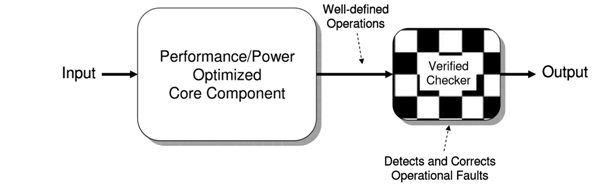
\includegraphics[width=10cm]{btwc.png}
		\end{center}
		\caption{Better Than Worst Case Design Concept\cite{austin}
		\label{fig:btwc}}
	\end{figure}
	\subsection{Dynamic Voltage Scaling - Razor Logic}
	Decreasing the supply voltage is the most efficient way to lower the energy consumption. Implementing this, however, can lead into wrong calculation results because of delays. Therefore you have to check wether the result you get are correct or not. 
	The Razor Logic implements this by appending appending a control logic right after the main logic like in figure~\ref{fig:razor}. The logic consists of a main flip-flop and a shadow latch, a comperator and a switch. The output of the main flip-flop is connected to the next stage of calculation and to a XOR gate as well as the output of the shadow latch. The XOR gate controlls the switch, which toggles between the logic input and the output of the shadow latch.
	\newline
	The main flip-flop is controlled by the main clock, which goes faster than under the worst case. The shadow latch, however, depends on a shadow clock, that is delayed to the main one to manage the worst case. The main flip-flip saves the input signal only on a rising clock. When the result from the logic will be recieved in time, the main flip-flop will store it on the next rising clock. Likewise, the shadow latch will store the same result during a delayed high clock signal. Because of this, the input signals of the XOR gate are equal and no error occured. But when the calculation was too slow due to a low voltage supply, the results could differ. Eventhough the main flip flop could store a wrong result on rising clock, the shadow latch will look after this. In that case, the input signals of the XOR gate can differ, so an error occurs. As this happens, the state from the shadow latch will be passed to the input of the main flip flop for the next clock.\cite{austin}\cite{chinese}\cite{book}
	\begin{figure}[ht]
		\begin{center}
			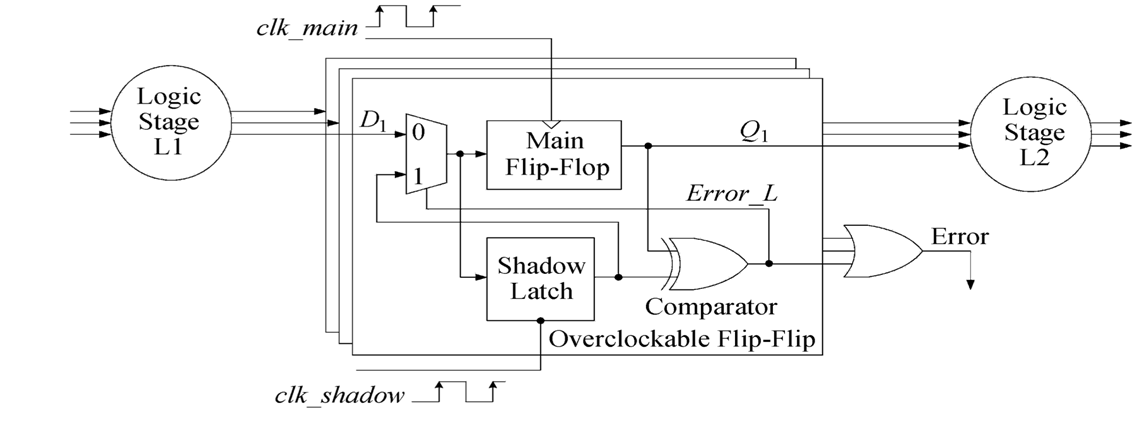
\includegraphics[width=12cm]{razor.png}
		\end{center}
		\caption{Razor Logic\cite{chinese}
			\label{fig:razor}}
	\end{figure}
	\newline
	Besides the logic, the error signal signal will also be passed to the pipeline stages. The reason for this is the avoidance of corrupted data in all the stages. To back this up, there are two different concepts\cite{book}: 
	\begin{enumerate}
		\item Clock Gating, like in figure~\ref{fig:cgate}, stalls the memory storage process after an error signal for one clock cycle. So the correct state can be passed from the shadow latch to the main flip flop. Then the pipeline continues normaly.
		\item Counterflow, like in figure~\ref{fig:cflow}, avoids stalling the pipeline for one clock. This will be used, when waiting is not possible due to an aggrissve pipeline design. The error signal, instead, is causing a bubble signal, which will be flushed thorugh the pipeline stages without any processing. After this the execution stage will be processed again.
	\end{enumerate} 
	\begin{figure}[ht]
		\begin{center}
			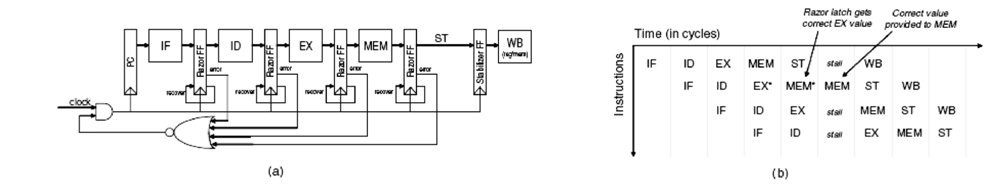
\includegraphics[width=14cm]{cgate.png}
		\end{center}
		\caption{Clock Gating\cite{picr}
			\label{fig:cgate}}
	\end{figure}
	\begin{figure}[ht]
		\begin{center}
			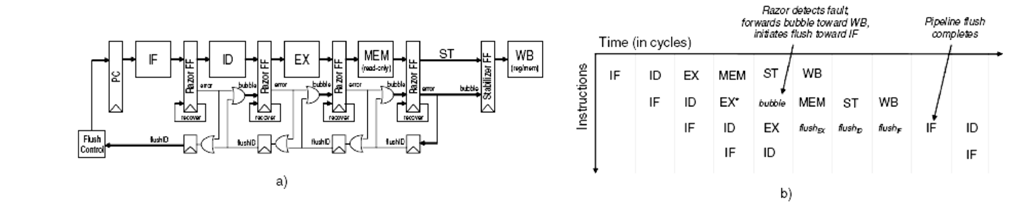
\includegraphics[width=14cm]{cflow.png}
		\end{center}
		\caption{Counterflow\cite{picr}
			\label{fig:cflow}}
	\end{figure}
	Finally, to adapt the voltage dynamically, you need a controlling system, that adapts the current voltage to the error signal. Such a controlling process is outlined in figure~\ref{fig:sum}. The error signals from the processing step are summed up to a sample error rate, which is compared to a reference one, e.g. 0\%. Based on this, a voltage control function regulates the voltage for the pipeline.
	\begin{figure}[ht]
		\begin{center}
			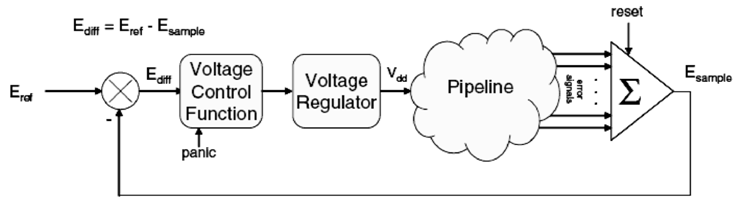
\includegraphics[width=10cm]{sum.png}
		\end{center}
		\caption{Dynamic voltage scaling process\cite{picr}
			\label{fig:sum}}
	\end{figure}
	\newline
	Mainly, the Razor is logic combined with dynamic voltage regulation to compensate environmental influencens as well as production ones. Apart from that, it can be used to go beyond the worst case specification for the voltage supply in runtime.
	In 2004 this system was tested on modified ARM cores with the SPEC2000 benchmark. The logic reached great energy savings up to 64\% by only producing 3\% overhead for error correction.\cite{picr}
	\subsection{Typical Case Optimization}
	Another important approach, to face the worst case design, is called Typical Case Optimization. In opposite to the Worst Case design, the TCO tries to adapt the logic to the typical case with a greater penalty in the worst case scenario. In fact the Razor logic is already a TCO solution, because less used parts of the electronic circuits will get a lower voltage supply at runtime.
	There are 3 steps to implement the TCO\cite{austin}: 
	\begin{enumerate}
		\item Evaluation of the duration under typical conditions, e.g. with example data
		\item Comparison to the general/random case
		\item Optimization of the circuits
	\end{enumerate}
	
	\begin{figure}[ht]
		\centering
		\begin{tabular}{ll}
			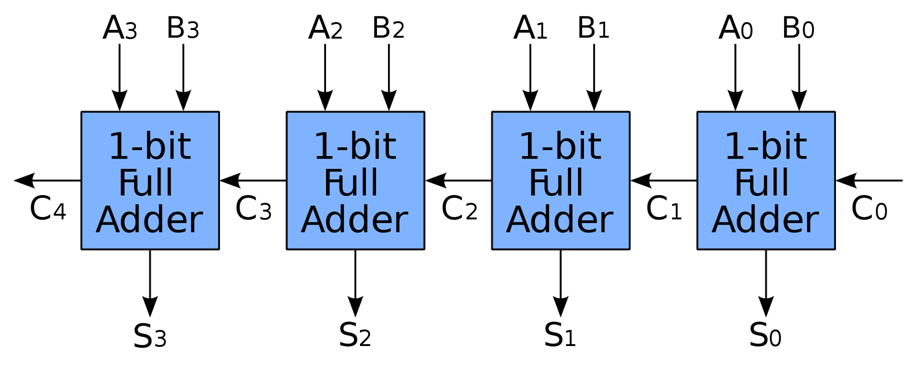
\includegraphics[width=7cm]{ripple.png}
			%\caption{Ripple Carry Adder ~\href{https://upload.wikimedia.org/wikipedia/commons/thumb/5/5d/4-bit_ripple_carry_adder.svg/2000px-4-bit_ripple_carry_adder.svg.png}{link} \label{fig:ripple}}
			&
				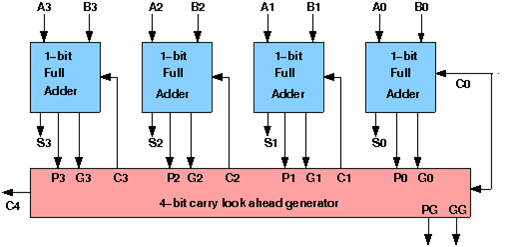
\includegraphics[width=7cm]{look.png}
			%\caption{Carry Look Ahead Adder ~\href{http://sit.iitkgp.ernet.in/~coavl/images/carrylookahead.png}{link} \label{fig:look}}
		\end{tabular}
		\caption{Ripple Carry Adder ~\href{https://upload.wikimedia.org/wikipedia/commons/thumb/5/5d/4-bit_ripple_carry_adder.svg/2000px-4-bit_ripple_carry_adder.svg.png}{link} \label{fig:ripple} and Carry Look Ahead Adder ~\href{http://sit.iitkgp.ernet.in/~coavl/images/carrylookahead.png}{link}}
	\end{figure}%
	
	To illustrate this process deeper in detail, a Ripple Carry adder will be analysed and implemented in a Carry Look Ahead one\cite{austin}, like in figure~\ref{fig:ripple}. A Ripple Carry adder consist of n 1 bit full adder, which are connected through the carry in/out. Even though the n single bits can be added in parallel, the whole adder has to wait for n carry in/out to ensure the correct result, shown in figure~\ref{fig:ripple}. But indeed, the Most Significant Bits have a higher impact on the results than the least ones. This is the reason why a TCO analysis should be done on the carry propagation. If the distances are far in the typical case, a special logic, e.g. a Carry Look Ahead adder, can be added. It will prefer them, vice versa for short distances. Therefore, the propagations for every bit position were evaluated within the SPEC2000 benchmark for typical sets of Add, Branch, Load and Store instructions. The same analysis was made with completely random data again to compare both and they can be found in figure~\ref{fig:pres} .  
	\begin{figure}[ht]
		\centering
		\begin{tabular}{ll}
			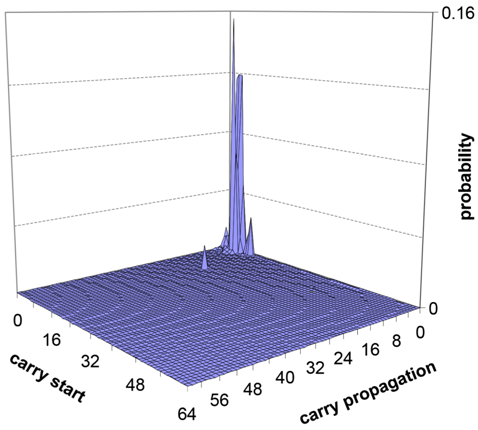
\includegraphics[width=6cm]{pres.png}
			%\caption{Ripple Carry Adder ~\href{https://upload.wikimedia.org/wikipedia/commons/thumb/5/5d/4-bit_ripple_carry_adder.svg/2000px-4-bit_ripple_carry_adder.svg.png}{link} \label{fig:ripple}}
			&
			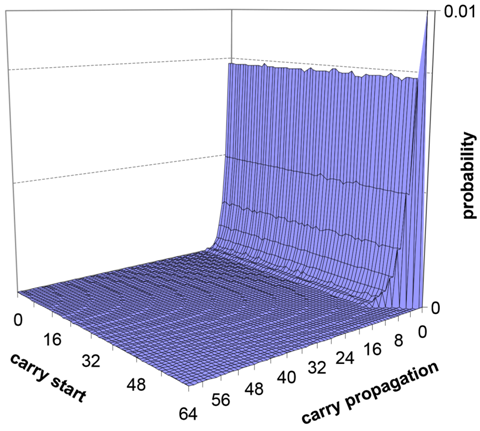
\includegraphics[width=6cm]{prand.png}
			%\caption{Carry Look Ahead Adder ~\href{http://sit.iitkgp.ernet.in/~coavl/images/carrylookahead.png}{link} \label{fig:look}}
		\end{tabular}
		\caption{Typical set (left) \label{fig:pres} and random set (right)\cite{austin}}
	\end{figure}%
	
	\begin{figure}[ht]
		\begin{center}
			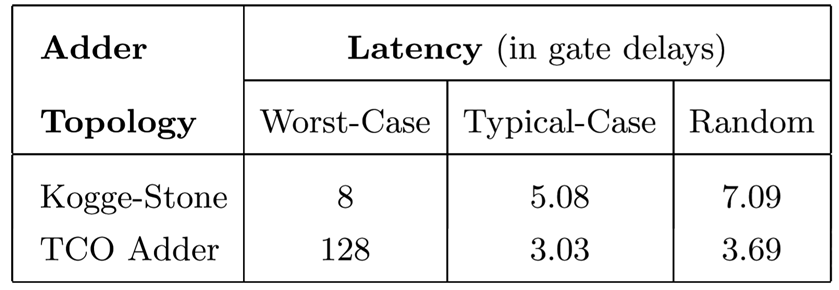
\includegraphics[width=7cm]{pcomp.png}
		\end{center}
		\caption{Comparison of TCO and Kogge Stone adder\cite{austin}
			\label{fig:pcomp}}
	\end{figure}
	As a result, the typical data set has mostly short carry propagation distances: in the least significant bits less then 6 and in the most significant bits more than 2. Whereas in the random set of data the propagation is independent from the bit position. As a consequence from these result, an optimized version of the adder was build as a Carry Look Ahead and compared to an Kogg-Stone adder, which is already optimized for the worst case. Table~\ref{fig:pcomp} shows the comparison between both of them. The optimized version has a very high latency compared to the Kogg-Stone adder in the worst case, but in the typical and even in the random case the TCO implementation is rather faster than the Kogg-Stone, which is a huge performance gain.\cite{austin}
	\subsection{Approximate Computing Designs}
	The last method that will be presented is the Approximate Computing Design. In contrast to the previous ones, this concept allows an error rate above 0\%. Therefore this approach is common used in AI or video applications where a lack of presicion is tolerable without any bigger impact on the results. There are 3 different ways to implement this design:\cite{chinese} 
	\newline
	Error Distribution Manipulation tries to reduce the energy consumption by reaching a specific error rate while lowering the voltage supply. A Ripple Carry Adder has a moderate error rate once the critical voltage supply was hit. Therefore this one good, if a moderate error rate is tolerated. 
	Apart from that, the Kogge Stone Adder has a lower critical voltage than the other one, but after reaching it, the error rate grows rapidly. So it should not be used for any error rate above 0 at all. 
	Because of these behaviours, the right method should be used at runtime considering the desired error rate.	By implementing this Method in the Kernel of the H.264 video codec, energy savings from 20\% up to 60\%.\cite{chinese}
	\newline
	The second method, Probabilistic Pruning, focuses on reducing less likely active parts of the electrical circuits. To get those, first of all the probability for the usage of any of them will be calculated based on simulations oder mathematical models. Then those circuits will be reduced and the error rate will be calculated. If the rate is to high, the reducing process will be made undone, otherwise it will be continued.
	\newline
	The last method uses a configurable approximative adder to adapt the error rate to the quality and speed during runtime. Because the MSB has the biggest influence on the result at addition, guessing the MSB based on the few previous ones uses less carry out information. The MSB is also less likely to be influenced by more distant bits. Therefore a higher throughput can be reached. For instance, with this method JPEG coding could reach a 21\% higher throughput.\cite{chinese}
	\newline
	\section{Challenges}
	The Worst Case design is indeed a limiting factor for higher clock rates and less energy consumption. But otherwise, error free systems for critical sections would not exist. Better Than Worst Case designs, however, show that it is possible to go beyond those restrictions. Having the hardware implementations on the one hand side, we can still have an error free system. On the other hand side, allowing approximation on non critical sections achieves significant savings without any complex hardware implementation at all. But still it is hard to implement approximation in general purpose processors. Through both of these processes, adapting to runtime is a crucial thing.
	Besides this, Worst Case design does not mean your system cannot get faster without the BTWC design. In fact it is possible to gain a boost without any big adjustmens. E.g. if you are using your computer at home, you will often have similar and stable conditions, that are not beyond the worst case. Therefore it is possible to overclock some CPU and GPU without any problems. With special cooling it is also possible to go even further than 8 GHz.\footnote{\href{http://valid.canardpc.com/records.php}{Overclocking Ranking}}

	
	% References
	\bibliographystyle{plain}  % you can try 'alpha' or 'abbrv' instead of 'plain'
	\bibliography{paper} % references are found in the file `paper.bib`
	
\end{document}